\documentclass[10pt,a4paper,oneside]{article}

%-----------------------------------------------------------------------
% Packages
\usepackage[utf8]{inputenc}
\usepackage[italian]{babel}
\usepackage{amsmath}
\usepackage{amsfonts}
\usepackage{amssymb}
\usepackage{graphicx}
\usepackage{lmodern}
\usepackage[colorlinks]{hyperref}

%-----------------------------------------------------------------------
% Package configuration
\hypersetup{
 urlcolor = blue
}

%-----------------------------------------------------------------------
% Heading
\title{Specifica Progetto di Laboratorio}
\author{Programmazione ad Oggetti}
\date{a.a. 2023/24}

%-----------------------------------------------------------------------
% Document
\begin{document}
\maketitle

%-----------------------------------------------------------------------
\section{Introduzione}
L'obiettivo del progetto è sviluppare una simulazione di sensori, ad esempio sensori che rilevano temperatura, umidità, presenza di polveri sottili o altri fenomeni, utilizzando il linguaggio di programmazione C++ e il framework \href{https://www.qt.io/?hsLang=en}{Qt} per creare un'interfaccia grafica utente. In questa simulazione, gli utenti finali dell'applicazione devono essere in grado di definire nuovi sensori, modificare e cancellare quelli esistenti, oltre ad avviare una simulazione. Si incoraggia l'uso di design pattern appropriati, benché non sia obbligatorio. Il progetto potrà essere sviluppato da un \textbf{singolo studente} oppure da una \textbf{coppia di studenti} e dovrà richiedere \textbf{approssimativamente 50 ore di lavoro} complessivo individuale.

La GUI può  trarre liberamente ispirazione sia da applicazioni per sistemi desktop che app per sistemi mobile. Si potrà aderire ai \emph{design pattern} \emph{Model-View-Controller} o \emph{Model-View} per la progettazione architetturale della GUI. Qt include un insieme di classi \emph{view} che usano una architettura \emph{Model/View} per gestire la relazione tra i dati logici della GUI ed il modo in cui essi sono presentati all'utente della GUI. Il framework Qt è dotato di una documentazione completa e precisa che sarà la principale guida di riferimento nello sviluppo della GUI, oltre ad offrire l'IDE QtCreator ed il tool QtDesigner. L'applicazione potrà anche applicare \emph{design pattern} comunemente utilizzati in C++.

Il voto dell'esame scritto e la valutazione del progetto sono tra loro indipendenti ed entrambi concorrono a formare il voto finale dell'esame, il quale viene calcolato indicativamente come media pesata tra il voto della prova scritta, la quale ha un peso maggiore, e il corrispettivo numerico della valutazione del progetto. Vi è comunque un margine di flessibilità favorevole allo studente nella determinazione del voto finale, in cui rimarrà preponderante il voto dell'esame scritto. Sarà possibile riconsegnare il progetto mantenendo il voto dell'esame scritto e viceversa. Sarà possibile sostenere l'esame scritto senza aver consegnato il progetto e viceversa, tuttavia la valutazione del progetto avverrà solamente per studenti che abbiano superato l'esame scritto e si siano iscritti nella lista Uniweb per la registrazione del voto finale.


%-----------------------------------------------------------------------
\section{Vincoli}
Il progetto deve obbligatoriamente soddisfare i seguenti vincoli:
\begin{enumerate}
 \item essere un \textbf{lavoro originale} dello studente o della coppia di studenti
 \item essere interamente \textbf{scritto in C++}
 \item prevedere un'\textbf{interfaccia grafica} realizzata in Qt
 \item \textbf{compilare senza errori} sulla macchina virtuale fornita (sono tollerati, sebbene generalmente penalizzati, i \emph{warning} durante la compilazione)
 \item realizzare i principi di \textbf{incapsulamento e \emph{information hiding}} della buona programmazione ad oggetti: una classe deve astrarre un singolo concetto e includere tutti gli attributi e metodi di cui ha bisogno con opportuni livelli di visibilità
 \item mantenere una \textbf{separazione netta} tra il modello logico e l'interfaccia grafica, ovvero il codice del modello deve poter essere riutilizzabile senza dipendere dall'interfaccia; nulla vieta che il codice del modello utilizzi strumenti di Qt non legati all'interfaccia, come le funzioni di I/O o le classi per la gestione di JSON
 \item eseguire in maniera \textbf{efficiente e robusta}, senza errori a \emph{runtime}
 \item utilizzare il \textbf{polimorfismo in maniera non banale}; alcuni esempi di utilizzo \emph{banale} sono i distruttori virtuali, metodi \emph{getter} che restituiscono informazioni leggermente diverse a seconda dell'oggetto di invocazione, metodi \emph{getType} che restituiscono una stringa contenente il tipo dell'oggetto; per contro un utilizzo \emph{non banale} del polimorfismo si può ottenere con metodi che svolgono operazioni diverse a seconda del tipo dinamico della variabile polimorfa di invocazione, come costruire un \emph{widget} grafico diverso a seconda dell'oggetto da mostrare; molti \emph{design pattern} richiedono un utilizzo del polimorfismo non banale e possono pertanto fornire ottimi spunti
 \item implementare una \textbf{gerarchia di classi} per i sensori con almeno \textbf{tre classi concrete} per i progetti svolti singolarmente, o almeno \textbf{cinque classi concrete} per i progetti svolti in coppia
 \item consentire la \textbf{creazione, la ricerca, la modifica e la cancellazione} dei sensori, tali operazioni devono essere fruibili tramite interfaccia grafica
 \item realizzare la \textbf{persistenza dei dati} dei sensori in una qualsiasi forma per i progetti svolti singolarmente, o in un formato strutturato (JSON, XML, etc.) per i progetti svolti in coppia
 \item consentire, tramite l'interfaccia grafica, il \textbf{salvataggio e il caricamento di  un file di sensori} (come descritto al punto precedente) attraverso opportune finestre di dialogo: non è consentito l'utilizzo di percorsi di file di sensori cablati nel codice sorgente
 \item consentire, tramite interfaccia grafica, di \textbf{avviare una simulazione} per un sensore selezionato, simulando un certo numero di raccolte di dati; i dati dovranno essere quindi mostrati in maniera opportuna, ad esempio tramite QtCharts; non è necessario che la simulazione sia interattiva
 \item essere corredato di una \textbf{relazione} in formato pdf, in lingua italiana o inglese, di massimo 8 pagine con testo a 10pt che riporti:
 \begin{enumerate}
  \item nome, cognome e numero di matricola di tutti i componenti del gruppo (o del singolo autore in caso di progetto svolto singolarmente)
  \item una breve introduzione che descriva i sensori utilizzati
  \item la descrizione del modello logico
  \item la descrizione dell'utilizzo non banale del polimorfismo
  \item la descrizione del metodo utilizzato per la persistenza dei dati
  \item la descrizione delle funzionalità implementate
  \item la rendicontazione delle ore previste e di quelle effettivamente svolte
  \item solo per progetti svolti in coppia: la suddivisione delle attività progettuali
  \item solo per progetti riconsegnati: una sezione che riporta le modifiche apportate rispetto all'ultima consegna; in caso di riconsegna senza modifiche è preferibile aggiungere comunque questa sezione indicando che non ci sono state modifiche
 \end{enumerate}
 In caso di progetto di coppia, \textbf{le relazioni devono essere distinte}. Assieme al documento di specifiche viene fornito anche un modello commentato di relazione il cui utilizzo non è obbligatorio. Si suggerisce inoltre l'uso di \href{https://it.wikipedia.org/wiki/LaTeX}{LaTeX} per la redazione della relazione, il sistema di scrittura universalmente usato dagli informatici in ambito accademico.

La Fig.~\ref{fig:skeleton} mostra un esempio di struttura dell'interfaccia grafica.

\begin{figure}[t]
 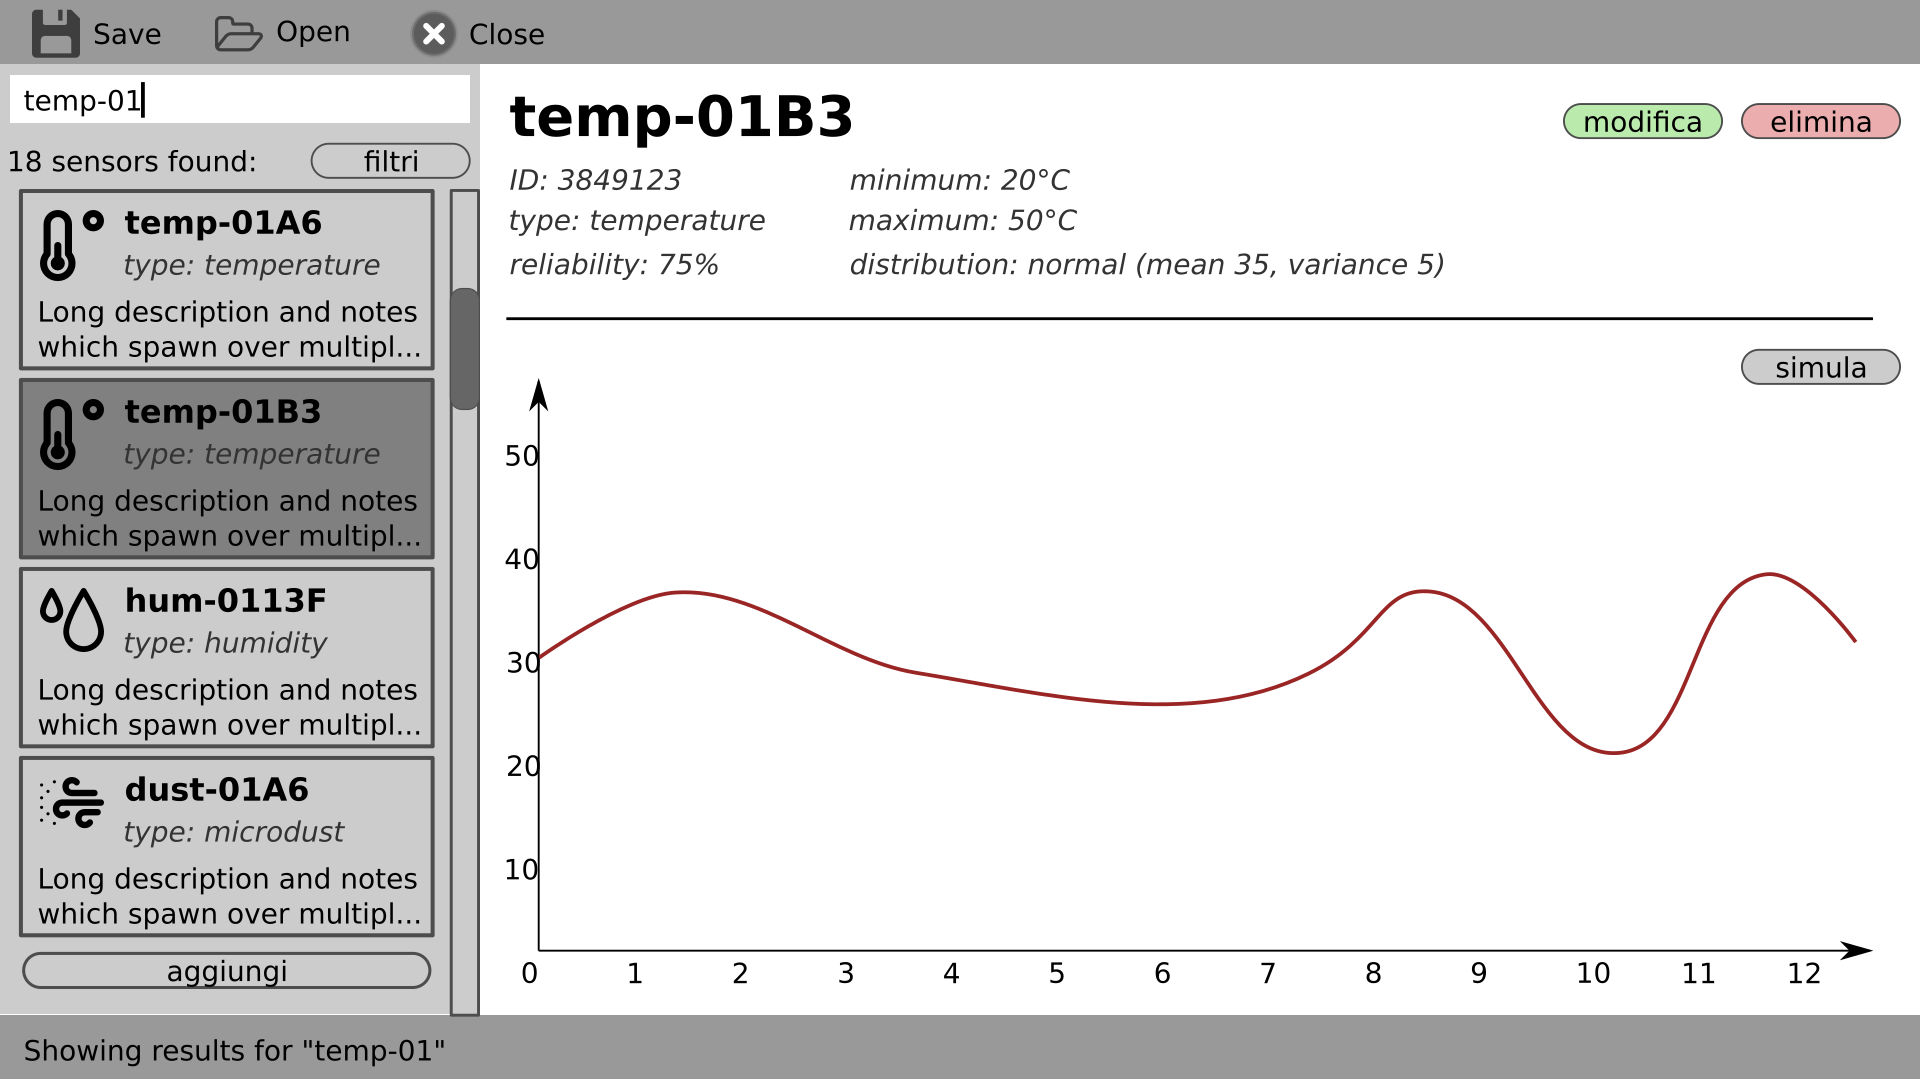
\includegraphics[width=0.95\textwidth]{assets/gui-skeleton-sample}
 \caption{Esempio di scheletro dell'interfaccia della finestra principale}\label{fig:skeleton}
\end{figure}
\end{enumerate}

%-----------------------------------------------------------------------
\section{Consegna}
La consegna avverrà tramite il Moodle del corso, all'interno del quale saranno attivate cinque sessioni di consegna del progetto per gli altrettanti appelli d'esame previsti durante l'anno accademico (due sessioni di consegna a gennaio/febbraio 2024, due sessioni di consegna a giugno/luglio 2024, 
una sessione di consegna a settembre 2024). Si dovrà consegnare un unico archivio in formato zip della dimensione massima di 256MB attraverso l'apposita pagina Moodle. \textbf{Non saranno accettati tentativi di consegna con modalità diverse o formati che non siano zip}. La cartella compressa dovrà contenere:
\begin{itemize}
 \item la relazione in formato PDF
 \item una sottocartella con i file sorgente del progetto (.h, .cpp, .pro, eventuali sottocartelle) ed eventuali file multimediali necessari (immagini, icone, ecc.)
 \item almeno un file d'esempio per la persistenza dei dati
\end{itemize}
La cartella \emph{non dovrebbe} contenere codice oggetto compilato, eseguibili, file generati dall'IDE o in generale qualsiasi file non utile ai fini della valutazione. Si raccomanda di verificare il corretto caricamento dei file su Moodle e di comunicare tempestivamente eventuali malfunzionamenti.

Nei progetti di coppia ogni studente dovrà provvedere separatamente alla propria consegna includendo il codice (lo stesso per i due membri della coppia) e la propria relazione (diversa per ciascuno). Se nella coppia solamente uno studente è sufficiente all'esame scritto, questo studente può comunque procedere alla consegna del progetto con l'obiettivo di finalizzare l'esame. Si ricorda che la valutazione del progetto con relativo feedback avverrà solamente per gli studenti sufficienti all'esame scritto ed iscritti alla lista uniweb per il voto finale.


%-----------------------------------------------------------------------
\section{Criteri di valutazione}
Il progetto viene valutato sulla base dei vincoli obbligatori e delle funzionalità implementate. Più precisamente, \textbf{se uno o più vincoli obbligatori non risultano soddisfatti il progetto verrà considerato insufficiente} e sarà necessaria una riconsegna in uno degli appelli successivi. Viceversa, \textbf{se tutti i vincoli obbligatori sono soddisfatti il progetto è considerato (almeno) sufficiente} e la valutazione aumenterà in base alla qualità delle funzionalità sviluppate e, in misura minore, in base alla qualità della relazione.

Una funzionalità viene valutata positivamente in base alla sua pertinenza al tema, all'utilità, all'usabilità, alla complessità e alla qualità del codice attraverso cui è implementata. Funzionalità più semplici o generiche migliorano la valutazione, sebbene non tanto quanto idee più complesse o articolate. Le scorciatoie da tastiera, per esempio, sono migliorie generiche semplici da ottenere con poche righe di codice in Qt, così come la gestione del ridimensionamento delle finestre o l'uso di icone. Per contro l'integrazione con un sistema di API o l'uso di basi di dati come SQL o MongoDB per la persistenza sono significativamente più complessi e richiedono la scrittura di classi apposite.

La qualità della relazione, pur avendo un'incidenza minore, verrà valutata sulla base della completezza, della chiarezza e della coesione. \textbf{Errori linguistici evidenti} come sistematica mancanza di punteggiatura o errori di battitura frequenti \textbf{verranno penalizzati}. È possibile redigere la relazione in Italiano o Inglese, a propria discrezione. La scelta della lingua non avrà effetti sulla valutazione.

Poiché il corso non tratta di usabilità o resa estetica della GUI la loro mancanza \textbf{non verrà penalizzata}, purché questo non pregiudichi il corretto funzionamento del programma. Tuttavia, se il progetto viene sviluppato ponendo particolare attenzione a queste caratteristiche, verrà riconosciuto un bonus come se si trattasse di una funzionalità aggiuntiva.

La valutazione del progetto è \textbf{valida per l'intero anno accademico} e fino a che non viene (ri)consegnato un progetto.

La valutazione è accompagnata da un feedback testuale che motiva la valutazione ed evidenzia i punti di forza e debolezza del progetto. È possibile riconsegnare un progetto per ottenere una nuova valutazione, che potrebbe anche essere peggiorativa, tuttavia se si seguono le indicazioni fornite dal feedback sarà generalmente migliorativa. La valutazione è \emph{idempotente}: riconsegnare lo stesso progetto senza modifiche produrrà esattamente lo stesso voto.

Consegnare un progetto svolto anche parzialmente da altri (con o senza il loro consenso) oppure generato da sistemi automatici comporta automaticamente l'insufficienza.

La registrazione del voto finale è possibile solo dopo:
\begin{itemize}
 \item avere superato con valutazione maggiore o uguale a 18 la prova scritta
 \item essersi iscritti alla lista Uniweb della per la registrazione del voto finale
 \item avere consegnato il progetto entro la scadenza prevista per la sessione in cui si intende verbalizzare il voto e aver ottenuto una valutazione positiva
\end{itemize}
Si ricorda che le liste Uniweb verificato il soddisfacimento delle propedeuticità e hanno una data di chiusura anticipata di almeno 5 giorni. Non saranno ammesse iscrizioni manuali in ritardo, per nessun motivo.

Il giorno della registrazione del voto finale previsto dalla corrispondente lista uniweb verrà inviato all'email istituzionale dei soli studenti iscritti alla lista uniweb il feedback relativo alla valutazione del progetto e verrà registrato su uniweb il voto finale complessivo dell'esame. In caso di valutazione negativa del progetto, l'esame non sarà superato: sarà quindi necessaria la riconsegna del progetto per una successiva scadenza di consegna; in questo caso il voto dell'esame scritto rimane comunque valido. Lo studente che rifiuterà il voto finale proposto via uniweb dovrà riconsegnare il progetto per una successiva scadenza di consegna (tranne all'ultimo appello d'esame, per cui ovviamente non esiste una successiva scadenza di consegna), cercando quindi di porre rimedio ai punti deboli segnalati nel feedback di valutazione e descrivendo obbligatoriamente le modifiche apportate al progetto nella relazione aggiornata; anche in questo caso il voto sufficiente dell'esame scritto rimane comunque valido. 



%-----------------------------------------------------------------------
\section{Note}
La parte di laboratorio dell'insegnamento di Programmazione a Oggetti ha una propria pagina ufficiale su GitHub all'indirizzo \href{https://github.com/Unipd-Object-Oriented-Programming}. Questo spazio contiene il materiale relativo a questo modulo dell'insegnamento, inclusi i lucidi delle lezioni e gli esempi del codice, suddivisi per anno accademico.

I video-tutorati dell'anno accademico 2020/2021 del tutor Benedetto Cosentino dedicati all'apprendimento delle caratteristiche di base del framework Qt per la progettazione di GUI sono disponibili su \href{https://www.youtube.com/playlist?list=PLH_Fd-836q-VcqWnnzsq3GOF2-0i_Az7p}{YouTube}.

\end{document}